\section{Problem Formulation}
\label{sec:problem}

This section presents the Mixed-Dimensional MAPF (MD-MAPF) formulation, the dimensional conflict taxonomy, and the execution model that bridges planning to real-time coordination.

\subsection{Mixed-Dimensional MAPF (MD-MAPF)}

\begin{definition}[MD-MAPF Instance]
A mixed-dimensional MAPF problem is defined as a tuple:
\begin{equation}
\mathcal{I} = (G, A, T, \kappa, \delta)
\end{equation}
where:
\begin{itemize}
    \item $G = (V, E)$ is a workspace graph with vertices $V$ and edges $E$
    \item $A = \{a_1, a_2, \ldots, a_n\}$ is a set of agents
    \item $T = \{t_1, t_2, \ldots, t_m\}$ is a set of tasks with deadlines
    \item $\kappa: A \rightarrow \{1, 2, 3\}$ is an agent dimensionality function
    \item $\delta: V \rightarrow \mathcal{P}(\{1, 2, 3\})$ is a vertex accessibility function
\end{itemize}
\end{definition}

The dimensionality function $\kappa(a)$ determines the operational space of each agent:

\begin{table}[htbp]
\centering
\caption{Agent Dimensionality Classification}
\label{tab:dimensionality}
\begin{tabular}{@{}cll@{}}
\toprule
$\kappa(a)$ & Type & Motion Space \\
\midrule
1 & Rail Robot & 1D linear path \\
2 & Mobile Robot & 2D planar surface \\
3 & Drone & 3D volumetric space \\
\bottomrule
\end{tabular}
\end{table}

\begin{definition}[Vertex Compatibility]
Agent $a$ can occupy vertex $v$ if and only if $\kappa(a) \in \delta(v)$.
\end{definition}

This formalizes that rail robots access only rail vertices, mobile robots access floor vertices, and drones access airspace vertices at appropriate altitude layers.

\begin{figure}[htbp]
\centering
% MD-MAPF Workspace: 1D rails, 2D floor, 3D airspace
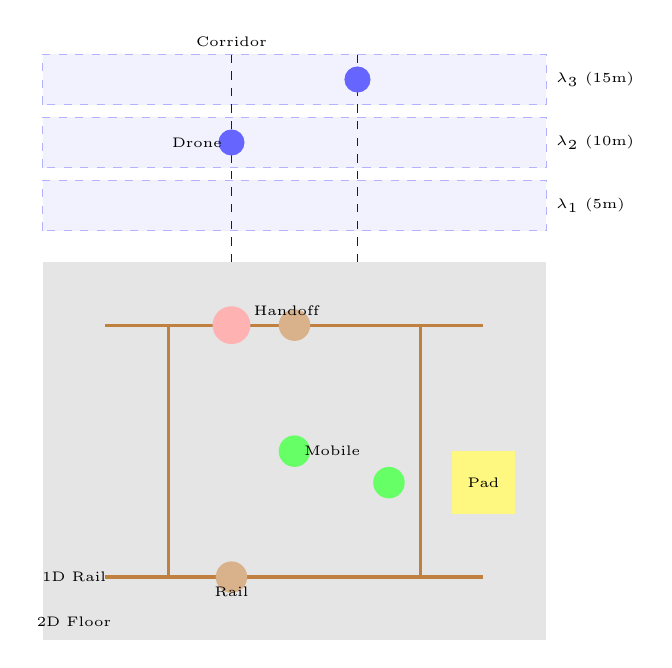
\begin{tikzpicture}[
    scale=0.8,
    rail/.style={very thick, brown},
    floor/.style={fill=gray!20},
    airspace/.style={fill=blue!5, draw=blue!30, dashed},
    agent1d/.style={fill=brown!60, circle, minimum size=0.4cm},
    agent2d/.style={fill=green!60, circle, minimum size=0.4cm},
    agent3d/.style={fill=blue!60, circle, minimum size=0.3cm}
]

% Floor (2D layer)
\fill[floor] (0,0) rectangle (8,6);
\node at (0.5, 0.3) {\tiny 2D Floor};

% Rails (1D)
\draw[rail] (1, 1) -- (7, 1);
\draw[rail] (1, 5) -- (7, 5);
\draw[rail] (2, 1) -- (2, 5);
\draw[rail] (6, 1) -- (6, 5);
\node at (0.5, 1) {\tiny 1D Rail};

% Airspace layers
\begin{scope}[yshift=6.5cm]
    \fill[airspace] (0, 0) rectangle (8, 0.8);
    \node[right] at (8, 0.4) {\tiny $\lambda_1$ (5m)};
    \fill[airspace] (0, 1) rectangle (8, 1.8);
    \node[right] at (8, 1.4) {\tiny $\lambda_2$ (10m)};
    \fill[airspace] (0, 2) rectangle (8, 2.8);
    \node[right] at (8, 2.4) {\tiny $\lambda_3$ (15m)};
\end{scope}

% Vertical corridors
\draw[dashed, blue] (3, 6) -- (3, 9.3);
\draw[dashed, blue] (5, 6) -- (5, 9.3);
\node at (3, 9.5) {\tiny Corridor};

% Agents
\node[agent1d] (r1) at (3, 1) {};
\node[agent1d] (r2) at (4, 5) {};
\node[agent2d] (m1) at (4, 3) {};
\node[agent2d] (m2) at (5.5, 2.5) {};
\node[agent3d] (d1) at (3, 7.9) {};
\node[agent3d] (d2) at (5, 8.9) {};

% Labels
\node[below] at (r1) {\tiny Rail};
\node[right] at (m1) {\tiny Mobile};
\node[left] at (d1) {\tiny Drone};

% Handoff point
\fill[red!30] (3, 5) circle (0.3);
\node[above right] at (3.2, 5) {\tiny Handoff};

% Charging pad
\fill[yellow!50] (6.5, 2) rectangle (7.5, 3);
\node at (7, 2.5) {\tiny Pad};

\end{tikzpicture}

\caption{MD-MAPF workspace showing 1D rails (brown), 2D floor (gray), 3D airspace layers ($\lambda_1$-$\lambda_3$), vertical corridors, handoff points, and charging pads.}
\label{fig:workspace}
\end{figure}

\subsection{Space-Time Representation}

\begin{definition}[Space-Time State]
For an agent of dimensionality $d$, the state in the space-time graph is:
\begin{equation}
s = (v, t, \lambda) \quad \text{where} \quad v \in V, t \in \mathbb{R}_{\geq 0}, \lambda \in \Lambda
\end{equation}
\end{definition}

The layer component $\lambda$ has dimension-specific semantics:
\begin{itemize}
    \item For $d = 1$: $\lambda$ is position on rail segment (continuous)
    \item For $d = 2$: $\lambda = \emptyset$ (not applicable)
    \item For $d = 3$: $\lambda \in \{0, 5, 10, 15\}$ meters (discrete altitude layers)
\end{itemize}

\begin{axiom}[Dimensionality Conservation]
An agent cannot change its dimensionality during execution:
\begin{equation}
\forall a \in A, \forall t_1, t_2 \in \mathbb{R}_{\geq 0}: \kappa(a, t_1) = \kappa(a, t_2)
\end{equation}
\end{axiom}

\begin{axiom}[Inter-Dimensional Transition]
An agent of dimension $d_1$ can interact with an agent of dimension $d_2$ only at vertices where their dimensions intersect:
\begin{equation}
\text{interact}(a_1, a_2, v) \Rightarrow \kappa(a_1) \in \delta(v) \land \kappa(a_2) \in \delta(v)
\end{equation}
\end{axiom}

\subsection{Dimensional Conflict Taxonomy}

Classical CBS~\cite{sharon2015cbs} treats all conflicts uniformly. We introduce a six-class taxonomy based on dimensional interaction, enabling specialized resolution strategies.

\begin{definition}[Dimensional Conflict]
Let $a_1, a_2 \in A$ be agents with dimensionalities $d_1 = \kappa(a_1)$ and $d_2 = \kappa(a_2)$. A conflict between them is classified by the pair $(d_1, d_2)$.
\end{definition}

\begin{table}[htbp]
\centering
\caption{Six-Class Dimensional Conflict Taxonomy}
\label{tab:conflicts}
\begin{tabular}{@{}clll@{}}
\toprule
Class & $(d_1, d_2)$ & Name & Description \\
\midrule
$C_1$ & $(1, 1)$ & \textsc{Linear} & Same rail segment \\
$C_2$ & $(2, 2)$ & \textsc{Planar} & 2D plane collision \\
$C_3$ & $(1, 2)$ & \textsc{Crossing} & Rail-floor intersection \\
$C_4$ & $(3, 3)$ & \textsc{Aerial} & Same airspace layer \\
$C_5$ & $(3, 3)$ & \textsc{Vertical} & Vertical corridor \\
$C_6$ & $(3, 1/2)$ & \textsc{Air-Ground} & Handoff point \\
\bottomrule
\end{tabular}
\end{table}

Each conflict class admits specialized resolution strategies that exploit dimensional structure, achieving significant pruning of the CBS search tree compared to uniform treatment.

\begin{figure}[htbp]
\centering
% Conflict Taxonomy: 6 conflict classes visual grid
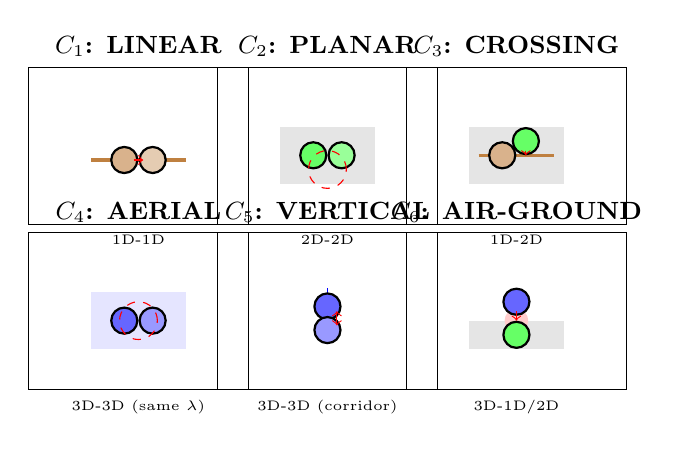
\begin{tikzpicture}[
    scale=0.6,
    box/.style={draw, minimum width=2.8cm, minimum height=2cm, align=center},
    agent/.style={circle, minimum size=0.3cm, draw, thick}
]

% Row 1
\node[box] (c1) at (0, 0) {};
\node[above] at (c1.north) {\small\textbf{$C_1$: LINEAR}};
\draw[brown, very thick] (-1, -0.3) -- (1, -0.3);
\node[agent, fill=brown!60] at (-0.3, -0.3) {};
\node[agent, fill=brown!40] at (0.3, -0.3) {};
\draw[red, ->] (-0.1, -0.3) -- (0.1, -0.3);
\node[below] at (c1.south) {\tiny 1D-1D};

\node[box] (c2) at (4, 0) {};
\node[above] at (c2.north) {\small\textbf{$C_2$: PLANAR}};
\fill[gray!20] (3, -0.8) rectangle (5, 0.4);
\node[agent, fill=green!60] at (3.7, -0.2) {};
\node[agent, fill=green!40] at (4.3, -0.2) {};
\draw[red, dashed] (4, -0.5) circle (0.4);
\node[below] at (c2.south) {\tiny 2D-2D};

\node[box] (c3) at (8, 0) {};
\node[above] at (c3.north) {\small\textbf{$C_3$: CROSSING}};
\fill[gray!20] (7, -0.8) rectangle (9, 0.4);
\draw[brown, very thick] (7.2, -0.2) -- (8.8, -0.2);
\node[agent, fill=brown!60] at (7.7, -0.2) {};
\node[agent, fill=green!60] at (8.2, 0.1) {};
\draw[red, ->] (8.2, -0.1) -- (8.2, -0.2);
\node[below] at (c3.south) {\tiny 1D-2D};

% Row 2
\node[box] (c4) at (0, -3.5) {};
\node[above] at (c4.north) {\small\textbf{$C_4$: AERIAL}};
\fill[blue!10] (-1, -4.3) rectangle (1, -3.1);
\node[agent, fill=blue!60] at (-0.3, -3.7) {};
\node[agent, fill=blue!40] at (0.3, -3.7) {};
\draw[red, dashed] (0, -3.7) circle (0.4);
\node[below] at (c4.south) {\tiny 3D-3D (same $\lambda$)};

\node[box] (c5) at (4, -3.5) {};
\node[above] at (c5.north) {\small\textbf{$C_5$: VERTICAL}};
\draw[blue, dashed] (4, -4.2) -- (4, -3);
\node[agent, fill=blue!60] at (4, -3.4) {};
\node[agent, fill=blue!40] at (4, -3.9) {};
\draw[red, <->] (4.2, -3.5) -- (4.2, -3.8);
\node[below] at (c5.south) {\tiny 3D-3D (corridor)};

\node[box] (c6) at (8, -3.5) {};
\node[above] at (c6.north) {\small\textbf{$C_6$: AIR-GROUND}};
\fill[gray!20] (7, -4.3) rectangle (9, -3.7);
\fill[red!20] (8, -3.7) circle (0.25);
\node[agent, fill=blue!60] at (8, -3.3) {};
\node[agent, fill=green!60] at (8, -4) {};
\draw[red, ->] (8, -3.5) -- (8, -3.7);
\node[below] at (c6.south) {\tiny 3D-1D/2D};

\end{tikzpicture}

\caption{Six-class dimensional conflict taxonomy. Each class has distinct resolution strategies based on the dimensional interaction between agents.}
\label{fig:conflicts}
\end{figure}

\subsection{Layered Airspace Model}

\begin{definition}[Airspace Layer]
The airspace is divided into discrete functional layers:
\begin{equation}
\Lambda = \{\lambda_0, \lambda_1, \lambda_2, \lambda_3\} = \{0\text{m}, 5\text{m}, 10\text{m}, 15\text{m}\}
\end{equation}
with operational semantics:
\begin{itemize}
    \item $\lambda_0$ (Ground): Landing, charging, handoff operations
    \item $\lambda_1$ (Handoff): Interaction with ground robots
    \item $\lambda_2$ (Work): Primary task execution layer
    \item $\lambda_3$ (Transit): Fast transit without conflicts
\end{itemize}
\end{definition}

\begin{definition}[Vertical Corridor]
A vertical corridor is a set of vertices $C \subset V$ such that:
\begin{equation}
\forall v \in C: \text{is\_corridor}(v) = \text{true}, \quad \forall \lambda \in \Lambda: \exists! v \in C: \text{layer}(v) = \lambda
\end{equation}
\end{definition}

Corridors are the exclusive transition points for layer changes.

\begin{definition}[Layer Transition Matrix]
The permitted layer transitions form matrix $\mathbf{T}$:
\begin{equation}
\mathbf{T} = \begin{bmatrix}
\checkmark & \checkmark & \times & \times \\
\checkmark & \checkmark & \checkmark & \times \\
\times & \checkmark & \checkmark & \checkmark \\
\times & \times & \checkmark & \checkmark
\end{bmatrix}
\end{equation}
where $T_{ij} = \checkmark$ indicates direct transition from $\lambda_i$ to $\lambda_j$ is permitted.
\end{definition}

\begin{axiom}[Corridor Exclusivity]
At any time, at most one drone can occupy a vertical corridor:
\begin{equation}
\forall C \in \text{Corridors}, \forall t: |\{a \in A : \text{position}(a, t) \in C\}| \leq 1
\end{equation}
\end{axiom}

\subsection{Energy Model}

\begin{definition}[Drone Energy State]
The drone state is extended with an energy component:
\begin{equation}
s = (v, t, \lambda, e) \quad \text{where} \quad e \in [0, E_{\max}]
\end{equation}
with $e$ representing remaining energy in Wh and $E_{\max}$ the battery capacity.
\end{definition}

\begin{definition}[Energy Consumption]
For action $\alpha$ with duration $\Delta t$:
\begin{equation}
\text{consume}(\alpha, \Delta t) = P(\alpha) \cdot \Delta t / 3600 \quad [\text{Wh}]
\end{equation}
where $P(\alpha)$ is action-specific power consumption:
\end{definition}

\begin{table}[htbp]
\centering
\caption{Drone Power Consumption Model}
\label{tab:power}
\begin{tabular}{@{}lc@{}}
\toprule
Action $\alpha$ & $P(\alpha)$ [W] \\
\midrule
\textsc{Hover} & 50 \\
\textsc{Move\_Horizontal} & 75 \\
\textsc{Climb} & 125 \\
\textsc{Descend} & 40 \\
\bottomrule
\end{tabular}
\end{table}

\begin{definition}[Path Energy Validity]
Path $\pi = [(v_0, t_0), \ldots, (v_k, t_k)]$ is energy-valid iff:
\begin{equation}
\forall i \in [1, k]: e_i = e_{i-1} - \text{consume}(\alpha_i, t_i - t_{i-1}) > 0
\end{equation}
with recharging at stations: if $\text{is\_charging\_pad}(v_i)$ then $e_i = E_{\max}$.
\end{definition}

\subsection{Deadline-Aware Execution Model}

To bridge planning to execution, we introduce deadline slack as a coordination signal.

\begin{definition}[Deadline Slack]
For task $t$ with deadline $d_t$, estimated duration $\tau_t$, at current time $t_{\text{now}}$:
\begin{equation}
\text{slack}(t) = d_t - (t_{\text{now}} + \tau_t)
\end{equation}
\end{definition}

\begin{definition}[Critical Task]
A task is critical when $\text{slack}(t) < \theta_{\text{critical}}$ (default 10 seconds).
\end{definition}

The slack value is normalized and published as a field component in the \ekkor{} execution layer, enabling gradient-based coordination where modules with tight deadlines naturally attract resources from neighbors with slack capacity.
